\thispagestyle{timhieukhoahocnone}
\pagestyle{timhieukhoahoc}
\everymath{\color{timhieukhoahoc}}
\blfootnote{\color{timhieukhoahoc}$^1$Đại học Osnabrueck, CHLB Đức.}
\graphicspath{{../timhieukhoahoc/pic2/}}
\begingroup
\AddToShipoutPicture*{\put(0,616){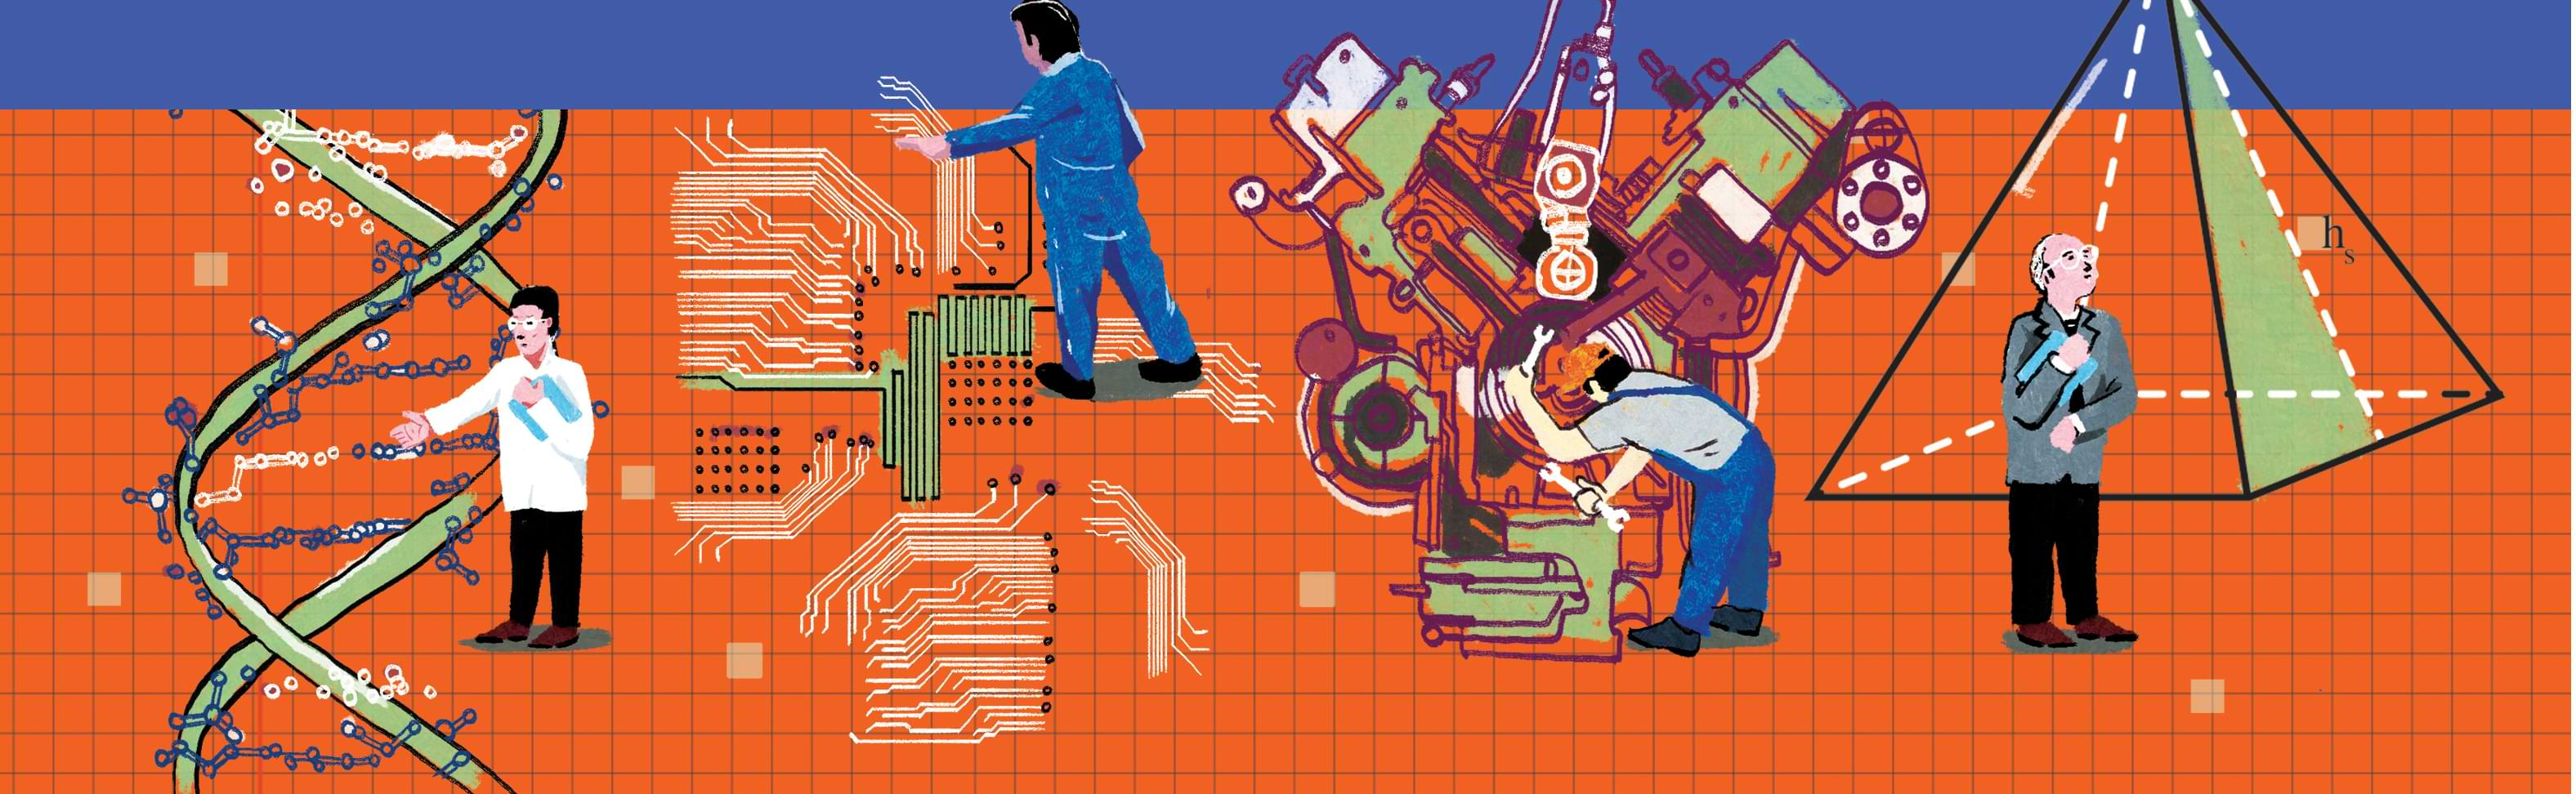
\includegraphics[width=19.3cm]{../bannertimhieu}}}
\AddToShipoutPicture*{\put(55,525){
\includegraphics[scale=0.95]{../tieude.pdf}}}
\centering
\endgroup
\vspace*{180pt}

\begin{multicols}{2}
	\textit{Vẻ đẹp của toán học nằm ở việc chứng minh các định lý. Cho đến thời điểm hiện tại, các nhà toán học vẫn chưa thể trông đợi vào những sự trợ giúp đến từ trí tuệ nhân tạo (AI). Tuy vậy, một chương trình có tên ``AlphaGeometry", được phát hành đầu năm $2024$ bởi một nhóm các nhà khoa học -- phần lớn là người Việt Nam -- hiện đang gây ngạc nhiên cho rất nhiều chuyên gia bởi khả năng của mình.}
	\vskip 0.1cm
	\textbf{\color{timhieukhoahoc}AlphaGeometry}
	\begin{figure}[H]
		\vspace*{-5pt}
		\centering
		\captionsetup{labelformat= empty, justification=centering}
		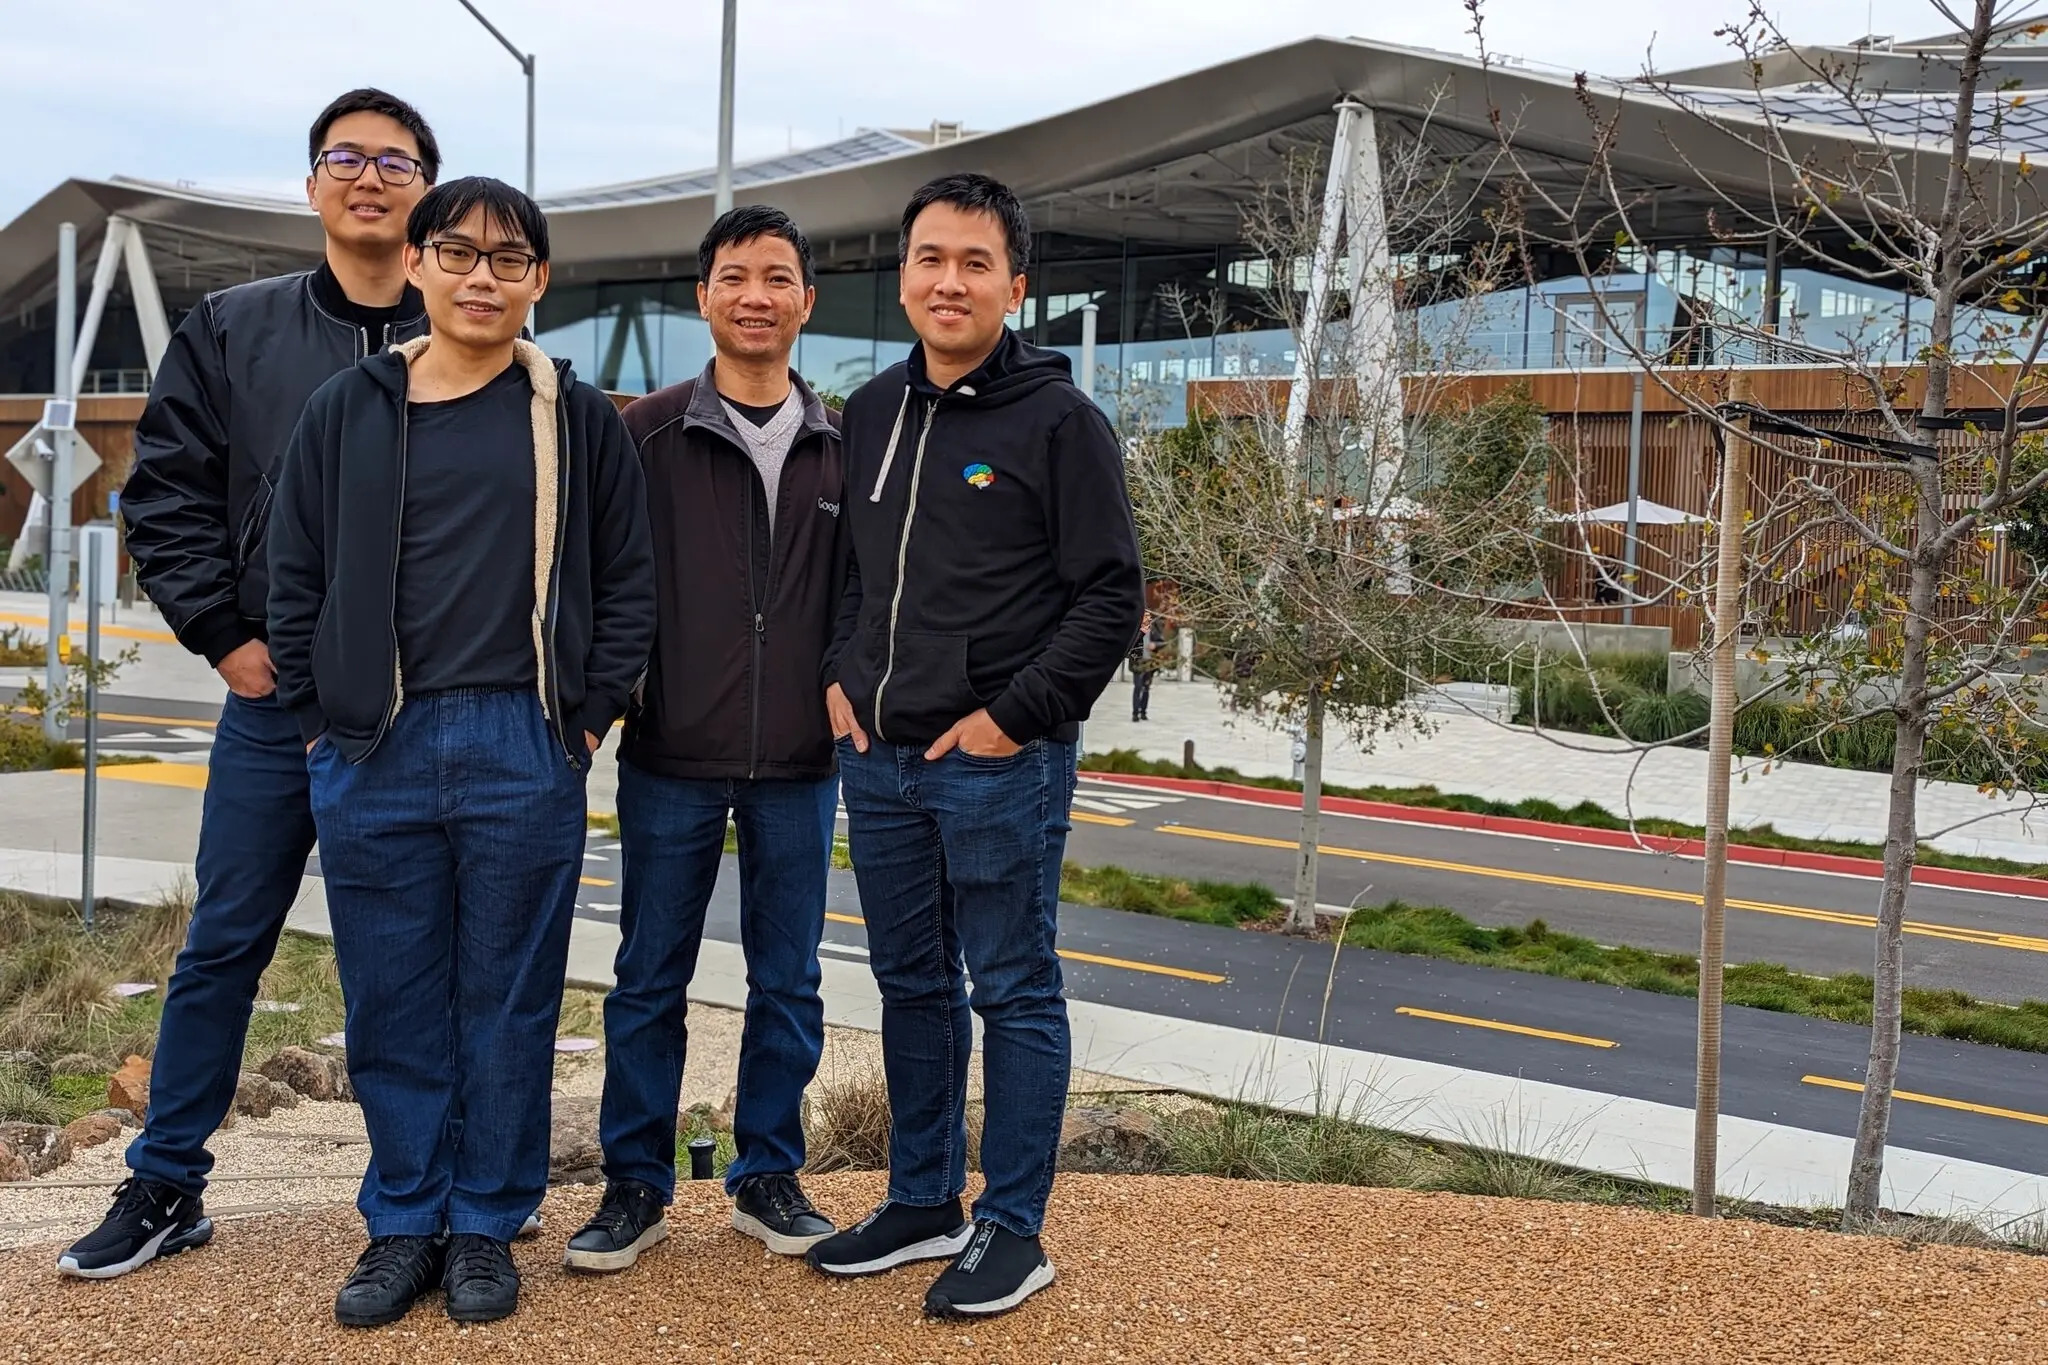
\includegraphics[width= 1\linewidth]{AlphaGeometry_team.jpg}
		\caption{\small\textit{\color{timhieukhoahoc}Hình $1$: Từ trái qua phải: Yuhuai Wu, Trịnh Hoàng Triều, Lê Viết Quốc và Lương Minh Thắng bên ngoài trụ sở của Google tại Mountain View, California.}}
		\vspace*{-10pt}
	\end{figure}
	Từ lâu, Olympic Toán học Quốc tế (IMO) được biết đến như kỳ thi toán học khó nhất dành cho học sinh phổ thông. Hàng năm, thí sinh từ khắp nơi trên thế giới đại diện cho các quốc gia tụ hội để cạnh tranh các huy chương đồng, bạc và vàng đáng mơ ước. Có thể không lâu nữa, các chương trình AI sẽ có đủ khả năng cạnh tranh với họ.
	\vskip 0.1cm
	Trong công trình xuất bản trên tạp chí Nature vào ngày $17$ tháng $1$ năm $2024$ vừa qua, một nhóm các nhà khoa học gồm TS. Trịnh Hoàng Triều  và GS. He He đến từ Đại học New York, TS. Yuhuai Wu đến từ xAI, TS. Lương Minh Thắng và TS. Lê Viết Quốc đến từ Google DeepMind, đã trình bày một chương trình AI mới có tên AlphaGeometry. Chương trình đã giải được $25$ trong số $30$ bài toán \textit{hình học} được rút ra từ các kỳ thi IMO từ năm $2000$ đến năm $2022$ và trình bày chúng dưới dạng mà con người có thể đọc được. Theo thống kê, những người đạt huy chương vàng giải được trung bình $25,9$ bài trong khoảng thời gian trên. Như vậy AI có khả năng giải quyết các bài toán hình học Olympiad ở mức độ gần bằng những thí sinh giỏi nhất, những người có thể giành được huy chương vàng trong cuộc thi. Hơn thế nữa, AlphaGeometry cũng đã tìm ra một lời giải tổng quát hơn cho một bài toán IMO năm $2004$ mà trước đó các chuyên gia đã bỏ qua. Khi nhóm nghiên cứu đưa các bài toán cho một hệ thống được phát triển vào những năm $1970$, được biết đến như là hệ thống chứng minh định lý hình học mạnh nhất (phương pháp Wu), thì chương trình chỉ giải quyết được $10$ bài toán.
	\vskip 0.1cm
	Trong vài năm qua, Google DeepMind đã theo đuổi một số dự án nghiên cứu ứng dụng AI đến toán học và đã đạt được một số kết quả. Tiêu biểu trong số đó là việc xây dựng các chương trình học máy hỗ trợ các nhà toán học trong việc kiểm chứng các giả thuyết trong lý thuyết biểu diễn và tổ hợp. Các công ty tiên phong khác như OpenAI và Meta AI cũng đã thu được những kết quả khả quan. Sự ra đời của AlphaGeometry đánh dấu bước nhảy vọt về khả năng của AI trong việc giải quyết các vấn đề hình học phức tạp.
	\vskip 0.1cm
	\textbf{\color{timhieukhoahoc}Chứng minh định lý hình học tự động}
	\vskip 0.1cm
	Là nền tảng của rất nhiều lĩnh vực như nghệ thuật, kiến trúc và kỹ thuật, hình học là khoa học nghiên cứu về không gian, khoảng cách, hình dạng và vị trí tương đối giữa các đối tượng. Trong suốt chiều dài lịch sử, con người luôn mong muốn có được những công cụ tổng quát để giải quyết các vấn đề hình học khác nhau. Khoảng hai nghìn năm trước, một vị vua Ai Cập đã hỏi Euclid rằng liệu có cách nào dễ dàng hơn để học hình học hay không. Câu trả lời của ông là: ``Không có con đường hoàng gia nào dẫn đến hình học". 
	\begin{figure}[H]
		\vspace*{-5pt}
		\centering
		\captionsetup{labelformat= empty, justification=centering}
		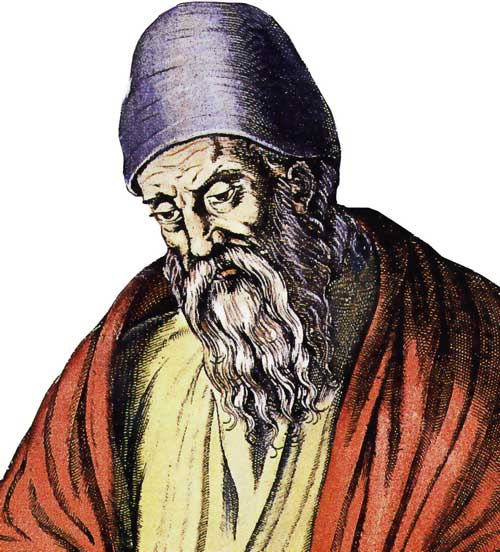
\includegraphics[width= 0.8\linewidth]{Euclid.jpg}
		\caption{\small\textit{\color{timhieukhoahoc}Hình $2$: Euclid. Nguồn: Britannica.}}
		\vspace*{-5pt}
	\end{figure}
	Tất nhiên, khó khăn ở đây không phải là các khái niệm hình học cơ bản như điểm, đường thẳng, góc, độ dài hay diện tích. Khó khăn nằm ở việc phát hiện ra các định lý thú vị và cách sử dụng lập luận logic để chứng minh chúng mà chỉ dựa trên một số tiên đề cho trước -- những phát biểu hiển nhiên đến mức có thể được coi là đương nhiên. Chúng ta có thể vẽ hàng chục hình tam giác với ba đường cao và thấy rằng ba đường cao của một tam giác cắt nhau tại cùng một điểm. Tuy nhiên, quan sát thực nghiệm chỉ là cơ sở để hình thành một phỏng đoán mà tính đúng đắn của nó phải được chứng minh bằng các phương tiện khác -- lý luận logic. 
	\vskip 0.1cm
	Ý tưởng chứng minh các định lý một cách cơ học đã xuất hiện từ thế kỷ $17$ bởi Leibniz và được hình thành dưới dạng toán học chính xác trong thế kỷ $20$ thông qua các công trình của Hilbert và những người theo trường phái logic toán học của ông. Về bản chất, chúng ta thay thế những khó khăn về mặt định tính vốn có trong các chứng minh toán học thông thường bằng sự phức tạp về mặt định lượng của các phép tính và về tiêu chuẩn hóa các quy trình chứng minh bằng thuật toán. 
	\vskip 0.1cm
	Từ những năm $1950$, với sự ra đời và phát triển của máy tính, những phép tính phức tạp về mặt định lượng mà trước đây vượt xa khả năng của con người như vậy dần trở nên tầm thường. Những chương trình chứng minh toán học tự động đã được phát triển dựa trên các hệ thống logic khác nhau (AI biểu tượng), nhằm giải quyết các bài toán một cách tự động. Chẳng hạn, \textit{Logic Theorist}, được phát triển bởi Allen Newell, Cliff Shaw và Herbert Simon vào năm $1955$, đã chứng minh được $38$ trong số $52$ định lý đầu tiên trong bộ sách \textit{Principia Mathematica} của Whitehead và Russell \footnote[2]{\color{timhieukhoahoc}``Máy tính và Trí tuệ nhân tạo", Pi số $12$ năm $2023$.}. 
	\vskip 0.1cm
	Tuy nhiên, bất chấp những nỗ lực mạnh mẽ, các nghiên cứu theo hướng này thường dẫn đến những vấn đề không thể giải quyết được bởi việc giải quyết các vấn đề hình học phụ thuộc rất nhiều vào các quy tắc do con người tạo ra. Mặc dù hiệu quả đối với các vấn đề đơn giản nhưng các công cụ biểu tượng lại gặp khó khăn về tính linh hoạt, đặc biệt khi phải đối mặt với các kịch bản hình học mới lạ hoặc độc đáo. 
	\vskip 0.2cm
	Việc giải quyết các vấn đề hình học thường đòi hỏi cả việc vận dụng các quy tắc logic và trực giác. Với mỗi bài toán, chúng ta thường phải xây dựng các cấu trúc bổ trợ như là thêm một đường thẳng, chia đôi một góc, vẽ một vòng tròn để tìm ra các mối liên hệ mới giữa các đối tượng. Việc không thể dự đoán các nhân tố ẩn hoặc các điểm phụ trợ quan trọng để chứng minh các bài toán hình học phức tạp làm nổi bật những hạn chế của các công cụ biểu tượng vốn chỉ dựa vào các quy tắc được xác định trước. Việc tạo ra các quy tắc toàn diện cho mọi tình huống có thể tưởng tượng được sẽ trở nên phi thực tế, dẫn đến các vấn đề về phạm vi bao phủ và khả năng mở rộng bị hạn chế.
	\vskip 0.2cm
	\textbf{\color{timhieukhoahoc}Sự trợ giúp đến từ AI}
	\vskip 0.2cm
	Với những tiến bộ mạnh mẽ gần đây trong lĩnh vực học máy -- cuộc cách mạng học sâu, những mô hình ngôn ngữ lớn sử dụng mạng thần kinh nhân tạo đã giúp con người giải quyết nhiều vấn đề trong xử lý ngôn ngữ tự nhiên như dịch thuật hay tạo văn bản tự động một cách thuyết phục. Về cơ bản, các mô hình này tạo ra văn bản bằng cách xuất ra các từ dần dần theo phân bố xác suất. Do lượng dữ liệu khổng lồ được đào tạo nên các chương trình AI như ChatGPT đôi khi có thể trả lời các câu hỏi một cách có ý nghĩa và thậm chí thực hiện các cuộc đối thoại giống con người. TS. Trịnh Hoàng Triều và nhóm của mình giờ đây đã có thể sử dụng cơ sở dữ liệu được xây dựng và tùy chỉnh để đào tạo AlphaGeometry với các bài toán và chứng minh toán học. 
	\vskip 0.1cm
	Tuy nhiên, do các mô hình ngôn ngữ lớn không học được các bước suy luận của một chứng minh nên công việc này cần được tiếp tục đảm nhận bởi một công cụ suy luận biểu tượng chuyên dụng. Với ý tưởng đó, AlphaGeometry kết hợp một mô hình ngôn ngữ với một công cụ biểu tượng -- một ``mạng thần kinh biểu tượng".
	\vskip 0.1cm
	Khi AlphaGeometry bắt đầu giải quyết một vấn đề, công cụ biểu tượng sẽ bắt đầu trước; nếu nó bị kẹt, mô hình ngôn ngữ sẽ đề xuất các xây dựng phụ trợ mới, mở ra những hướng suy luận mới cho công cụ biểu tượng. Vòng lặp tiếp tục cho đến khi kết luận được tìm thấy hoặc cho đến khi hết thời gian.
	\vskip 0.1cm
	Hình $3$ minh họa cách AlphaGeometry giải quyết một bài toán hình học đơn giản:
	\begin{figure}[H]
		\vspace*{-5pt}
		\centering
		\captionsetup{labelformat= empty, justification=centering}
		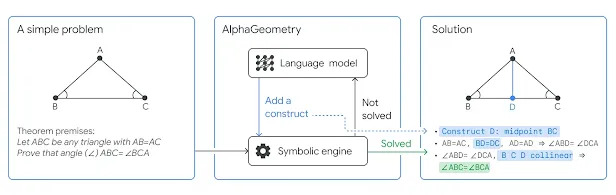
\includegraphics[width= 1\linewidth]{SimpleGeometry.jpg}
		\caption{\small\textit{\color{timhieukhoahoc}Hình $3$: Cách AlphaGeometry giải quyết vấn đề.}}
		\vspace*{-10pt}
	\end{figure}
	$a.$ Bài toán: Cho tam giác $ABC$ với $AB = AC$. Chứng minh rằng $\angle ABC = \angle BCA$.
	\vskip 0.1cm
	$b.$ AlphaGeometry trước tiên sử dụng công cụ suy luận biểu tượng để suy ra các phát biểu mới từ các giả thiết của bài toán cho đến khi kết luận được tìm thấy hoặc tất cả các phát biểu mới đã được sử dụng hết. 
	\vskip 0.1cm
	$c.$ Khi công cụ biểu tượng không tìm được chứng minh, mô hình ngôn ngữ của AlphaGeometry bổ sung thêm một cấu trúc có thể hữu ích, mở ra những hướng suy luận mới cho công cụ biểu tượng. Vòng lặp tiếp tục cho đến khi tìm được chứng minh.
	\vskip 0.1cm	
	$d.$ Trong ví dụ này, vòng lặp kết thúc sau cấu trúc phụ trợ đầu tiên ``$D$ là trung điểm của $BC$". Việc chứng minh bao gồm hai bước khác, cả hai đều sử dụng các thuộc tính ``$BD =DC$" và ``$B, D, C$ thẳng hàng", được tô màu xanh lam như trong hình.
	\vskip 0.1cm
	Phương pháp tiếp cận mạng thần kinh biểu tượng của AlphaGeometry phù hợp với lý thuyết quá trình kép, một khái niệm chia nhận thức của con người thành hai hệ thống - một hệ thống dành cho những ý tưởng nhanh chóng, trực quan và hệ thống còn lại dành cho việc ra quyết định hợp lý, có lý trí hơn. Các mô hình ngôn ngữ lớn vượt trội trong việc nhận dạng các mẫu chung nhưng thường thiếu lý luận hợp lý, trong khi các công cụ suy luận biểu tượng dựa trên các quy tắc rõ ràng nhưng có thể chậm và không linh hoạt. AlphaGeometry tận dụng điểm mạnh của cả hai hệ thống, với mô hình ngôn ngữ hướng dẫn công cụ suy luận biểu tượng đến các giải pháp khả thi. 
	\begin{figure}[H]
		\vspace*{-5pt}
		\centering
		\captionsetup{labelformat= empty, justification=centering}
		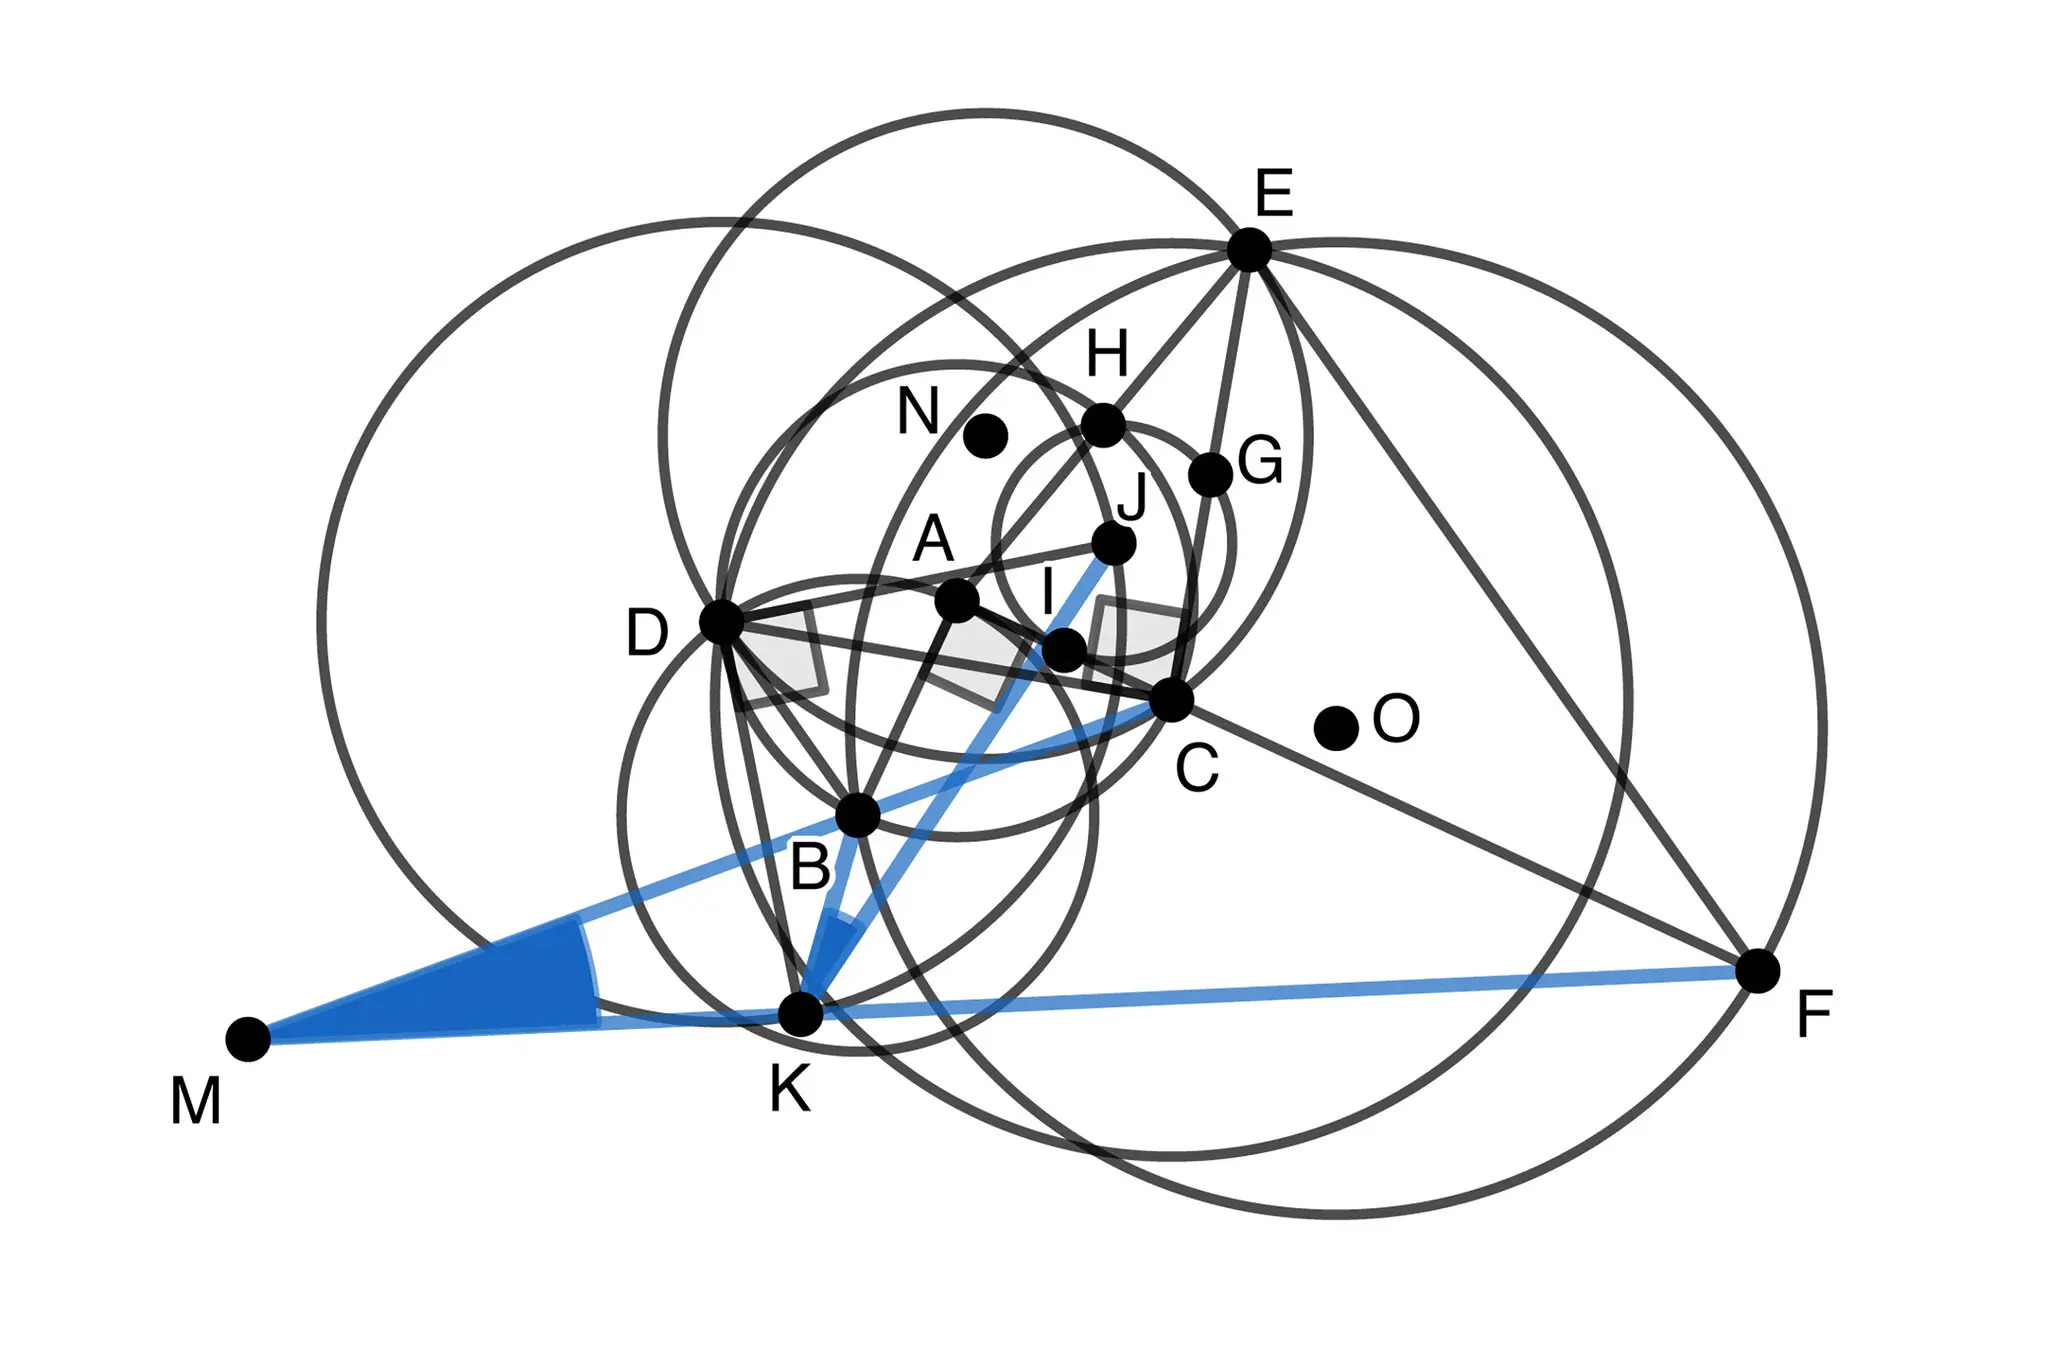
\includegraphics[width= 1\linewidth]{geometry.jpg}
		\caption{\small\textit{\color{timhieukhoahoc}Hình $4$: Một chứng minh phức tạp của AlphaGeometry có độ dài $247$ bước.}}
		\vspace*{-10pt}
	\end{figure}
	\textbf{\color{timhieukhoahoc}Tạo ra dữ liệu tổng hợp với $\pmb{100}$ triệu ví dụ}
	\vskip 0.1cm
	Cách tiếp cận phổ biến nhất hiện nay cho các vấn đề trong học máy là lấy dữ liệu được tạo ra bởi con người và tìm hiểu chúng thông qua học có giám sát. Sự thiếu hụt dữ liệu đào tạo là một trong những lý do chính cản trở việc áp dụng phương pháp này cho việc giải quyết các bài toán trừu tượng.
	\vskip 0.1cm
	Các mô hình ngôn ngữ lớn như GPT--$4$ được đào tạo với hàng chục Gigabyte tệp văn bản, tương ứng với khoảng $20$ triệu trang A$4$ được lấp đầy \footnote[3]{\color{timhieukhoahoc}Xem bài ``Dạy máy tính ngôn ngữ: Từ Google Translate đến ChatGPT" trên Pi số $1-2$ năm $2024$.}. Mặc dù có rất nhiều tài liệu về toán học nhưng việc dịch một chứng minh sang ngôn ngữ lập trình mà máy tính có thể hiểu được đòi hỏi rất nhiều công sức. Điều này đặc biệt khó khăn trong lĩnh vực hình học mà ở đó các chứng minh thường khó hình thức hóa hơn. Mặc dù có những ngôn ngữ lập trình được phát triển riêng cho hình học nhưng những ngôn ngữ này hầu như không sử dụng được các phương pháp từ các lĩnh vực khác. Chẳng hạn, nếu phép chứng minh yêu cầu một bước trung gian trong đó xuất hiện các số phức thì ngôn ngữ hình học này không thể được sử dụng. Bởi vậy nhóm nghiên cứu AlphaGeometry đã tạo ra bộ dữ liệu của riêng mình mà không cần phải dịch các chứng minh do con người viết sang ngôn ngữ hình thức.
	\vskip 0.1cm
	Trước tiên, các nhà khoa học tạo ra một tỷ sơ đồ ngẫu nhiên của các đối tượng hình học và rút ra tất cả mối quan hệ giữa các điểm và đường trong mỗi sơ đồ thông qua công cụ suy luận biểu tượng. Nói cách khác, AlphaGeometry tìm ra tất cả các chứng minh có trong mỗi sơ đồ. Sau đó chương trình truy ngược lại để tìm ra những cấu trúc bổ sung nào, nếu có, là cần thiết để đi đến những chứng minh đó. Quá trình này được gọi là ``suy luận biểu tượng và truy nguyên" (symbolic deduction and traceback).
	\vskip 0.1cm
	Chẳng hạn, một hình tam giác có chiều cao được vẽ và các điểm được đánh dấu bổ sung dọc theo các cạnh. Sau đó, các nhà nghiên cứu sử dụng thuật toán suy luận để suy ra các tính chất khác của tam giác, chẳng hạn như các góc tương ứng và đường thẳng nào vuông góc với nhau. 
	\vskip 0.1cm
	Tiếp theo, tập dữ liệu khổng lồ này được lọc để loại trừ các ví dụ tương tự, dẫn đến tập dữ liệu đào tạo cuối cùng gồm $100$ triệu ví dụ duy nhất có độ khó khác nhau, trong đó có $9$ triệu cấu trúc đặc trưng được bổ sung. Với rất nhiều ví dụ về cách các cấu trúc này dẫn đến chứng minh, mô hình ngôn ngữ của AlphaGeometry có thể đưa ra những gợi ý hữu ích cho các cấu trúc mới khi trình bày các bài toán hình học IMO.
	\begin{figure}[H]
		\vspace*{-5pt}
		\centering
		\captionsetup{labelformat= empty, justification=centering}
		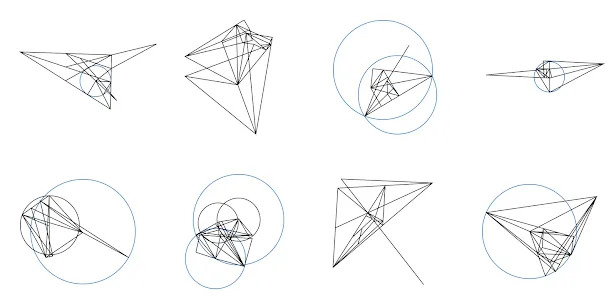
\includegraphics[width= 1\linewidth]{data_generated.jpg}
		\caption{\small\textit{\color{timhieukhoahoc}Hình $5$: Xây dựng dữ liệu cho AlphaGeometry.}}
		\vspace*{-10pt}
	\end{figure}
	Việc tạo ra dữ liệu tổng hợp đã giúp khắc phục được việc thiếu dữ liệu đào tạo. Theo GS. He He, lợi thế của việc không sử dụng các minh họa của con người là chương trình không bị hạn chế bởi các minh họa đó, do đó tạo cho mô hình một cơ hội để làm tốt hơn con người. Điều này gợi cho chúng ta nhớ đến AlphaZero, một chương trình AI chơi cờ vây được tạo ra mà không sử dụng dữ liệu từ các ván cờ của con người. Bằng cách tự chơi với chính mình, AlphaZero đã phát triển khả năng siêu việt và vượt qua phiên bản tiền nhiệm AlphaGo Lee với chiến thắng tuyệt đối $100 - 0$.
	\vskip 0.1cm
	\textbf{\color{timhieukhoahoc}Khả năng ấn tượng} 
	\vskip 0.1cm
	Lời giải của tất cả bài toán Olympic do AlphaGeometry cung cấp đều được máy tính kiểm tra và xác minh. Kết quả sau đó được so sánh với với các phương pháp AI trước đây và với thành tích của con người tại Olympic.
	\begin{figure}[H]
		\vspace*{-5pt}
		\centering
		\captionsetup{labelformat= empty, justification=centering}
		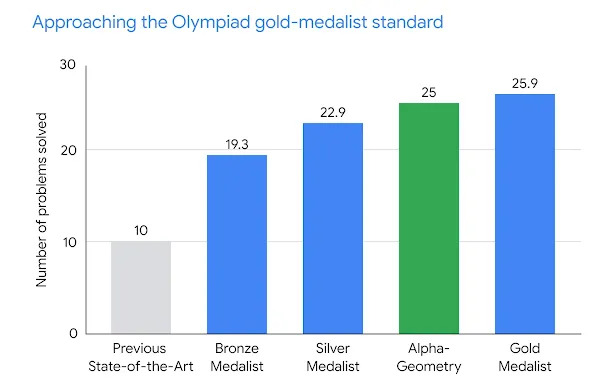
\includegraphics[width= 1\linewidth]{Results.jpg}
		\caption{\small\textit{\color{timhieukhoahoc}Hình $6$: So sánh kết quả của AlphaGeometry với các đối tượng khác nhau.}}
		\vspace*{-5pt}
	\end{figure}
	Evan Chen, một nghiên cứu sinh tiến sỹ ngành toán tại Viện Công nghệ Massachusetts (MIT) -- huy chương vàng IMO và cũng là một huấn luyện viên IMO của Mỹ -- sau khi đánh giá một số kết quả của AlphaGeometry cho biết: ``Kết quả của AlphaGeometry rất ấn tượng vì chúng rõ ràng và có thể kiểm chứng được. Các giải pháp AI trước đây cho các vấn đề đòi hỏi chứng minh trong các cuộc thi đôi khi không thành công (kết quả đầu ra nhiều khi không chính xác và cần có sự kiểm tra của con người). AlphaGeometry không có điểm yếu này: các lời giải của nó có cấu trúc có thể xác minh được bằng máy cũng như có thể đọc được bởi con người. Người ta có thể tưởng tượng ra một chương trình máy tính có thể giải các bài toán hình học bằng các hệ tọa độ cưỡng bức (Brute Force) sử dụng các tính toán đại số tẻ nhạt dài lê thê. AlphaGeometry không phải vậy. Chương trình sử dụng các quy tắc hình học cổ điển với các góc và các hình tam giác bằng nhau, tựa như cách học sinh làm."
	\vskip 0.1cm
	Cùng quan điểm trên, Peter Scholze -- giáo sư Toán tại Đại học Bonn, giải thưởng Fields $2018$ và $3$ lần giành huy chương vàng tại IMO -- cho rằng ``phương pháp giải các bài toán của AlphaGeometry nghe có vẻ hợp lý và ở một khía cạnh nào đó tương tự như việc đào tạo những người tham gia Olympic Toán Quốc tế."
	\vskip 0.1cm
	Terence Tao, nhà toán học tại Đại học California, Los Angeles -- giải thưởng Fields, là thí sinh trẻ nhất từ trước đến nay giành huy chương vàng IMO khi mới $12$ tuổi -- cho rằng AlphaGeometry là ``công trình tuyệt vời" và đã đạt được ``kết quả mạnh mẽ đáng ngạc nhiên". Ông nói, việc tinh chỉnh hệ thống AI. để giải quyết các vấn đề của Olympiad có thể không cải thiện kỹ năng nghiên cứu sâu của nó, nhưng trong trường hợp này, hành trình có thể có giá trị hơn đích đến.
	\vskip 0.1cm
	Mặc dù được xây dựng dựa trên sự mô phỏng cách con người giải quyết các bài toán hình học, lời giải của AlphaGeometry đôi khi rất khác với cách chúng ta giải chúng. Đầu tháng $12$ năm $2023$, TS. Lương Minh Thắng đã đến thăm trường cũ của mình là Trường Phổ thông năng khiếu, Đại học Quốc gia Thành phố Hồ Chí Minh và đưa AlphaGeometry cho giáo viên cũ của mình là TS. Lê Bá Khánh Trình. Là huấn luyện viên đội tuyển IMO của Việt Nam, TS. Lê Bá Khánh Trình từng đoạt huy chương vàng với điểm số tuyệt đối tại IMO $1979$ tại London, đồng thời giành giải đặc biệt cho bài giải hình học tinh tế của mình. TS. Lê Bá Khánh Trình đã phân tích một trong những cách chứng minh của AlphaGeometry và thấy nó đáng chú ý nhưng chưa thỏa đáng. TS. Lương Minh Thắng nhớ lại: ``Thầy thấy nó máy móc và cho rằng nó thiếu linh hồn, vẻ đẹp của một giải pháp mà ông đang tìm kiếm".
	\begin{figure}[H]
		\vspace*{-5pt}
		\centering
		\captionsetup{labelformat= empty, justification=centering}
		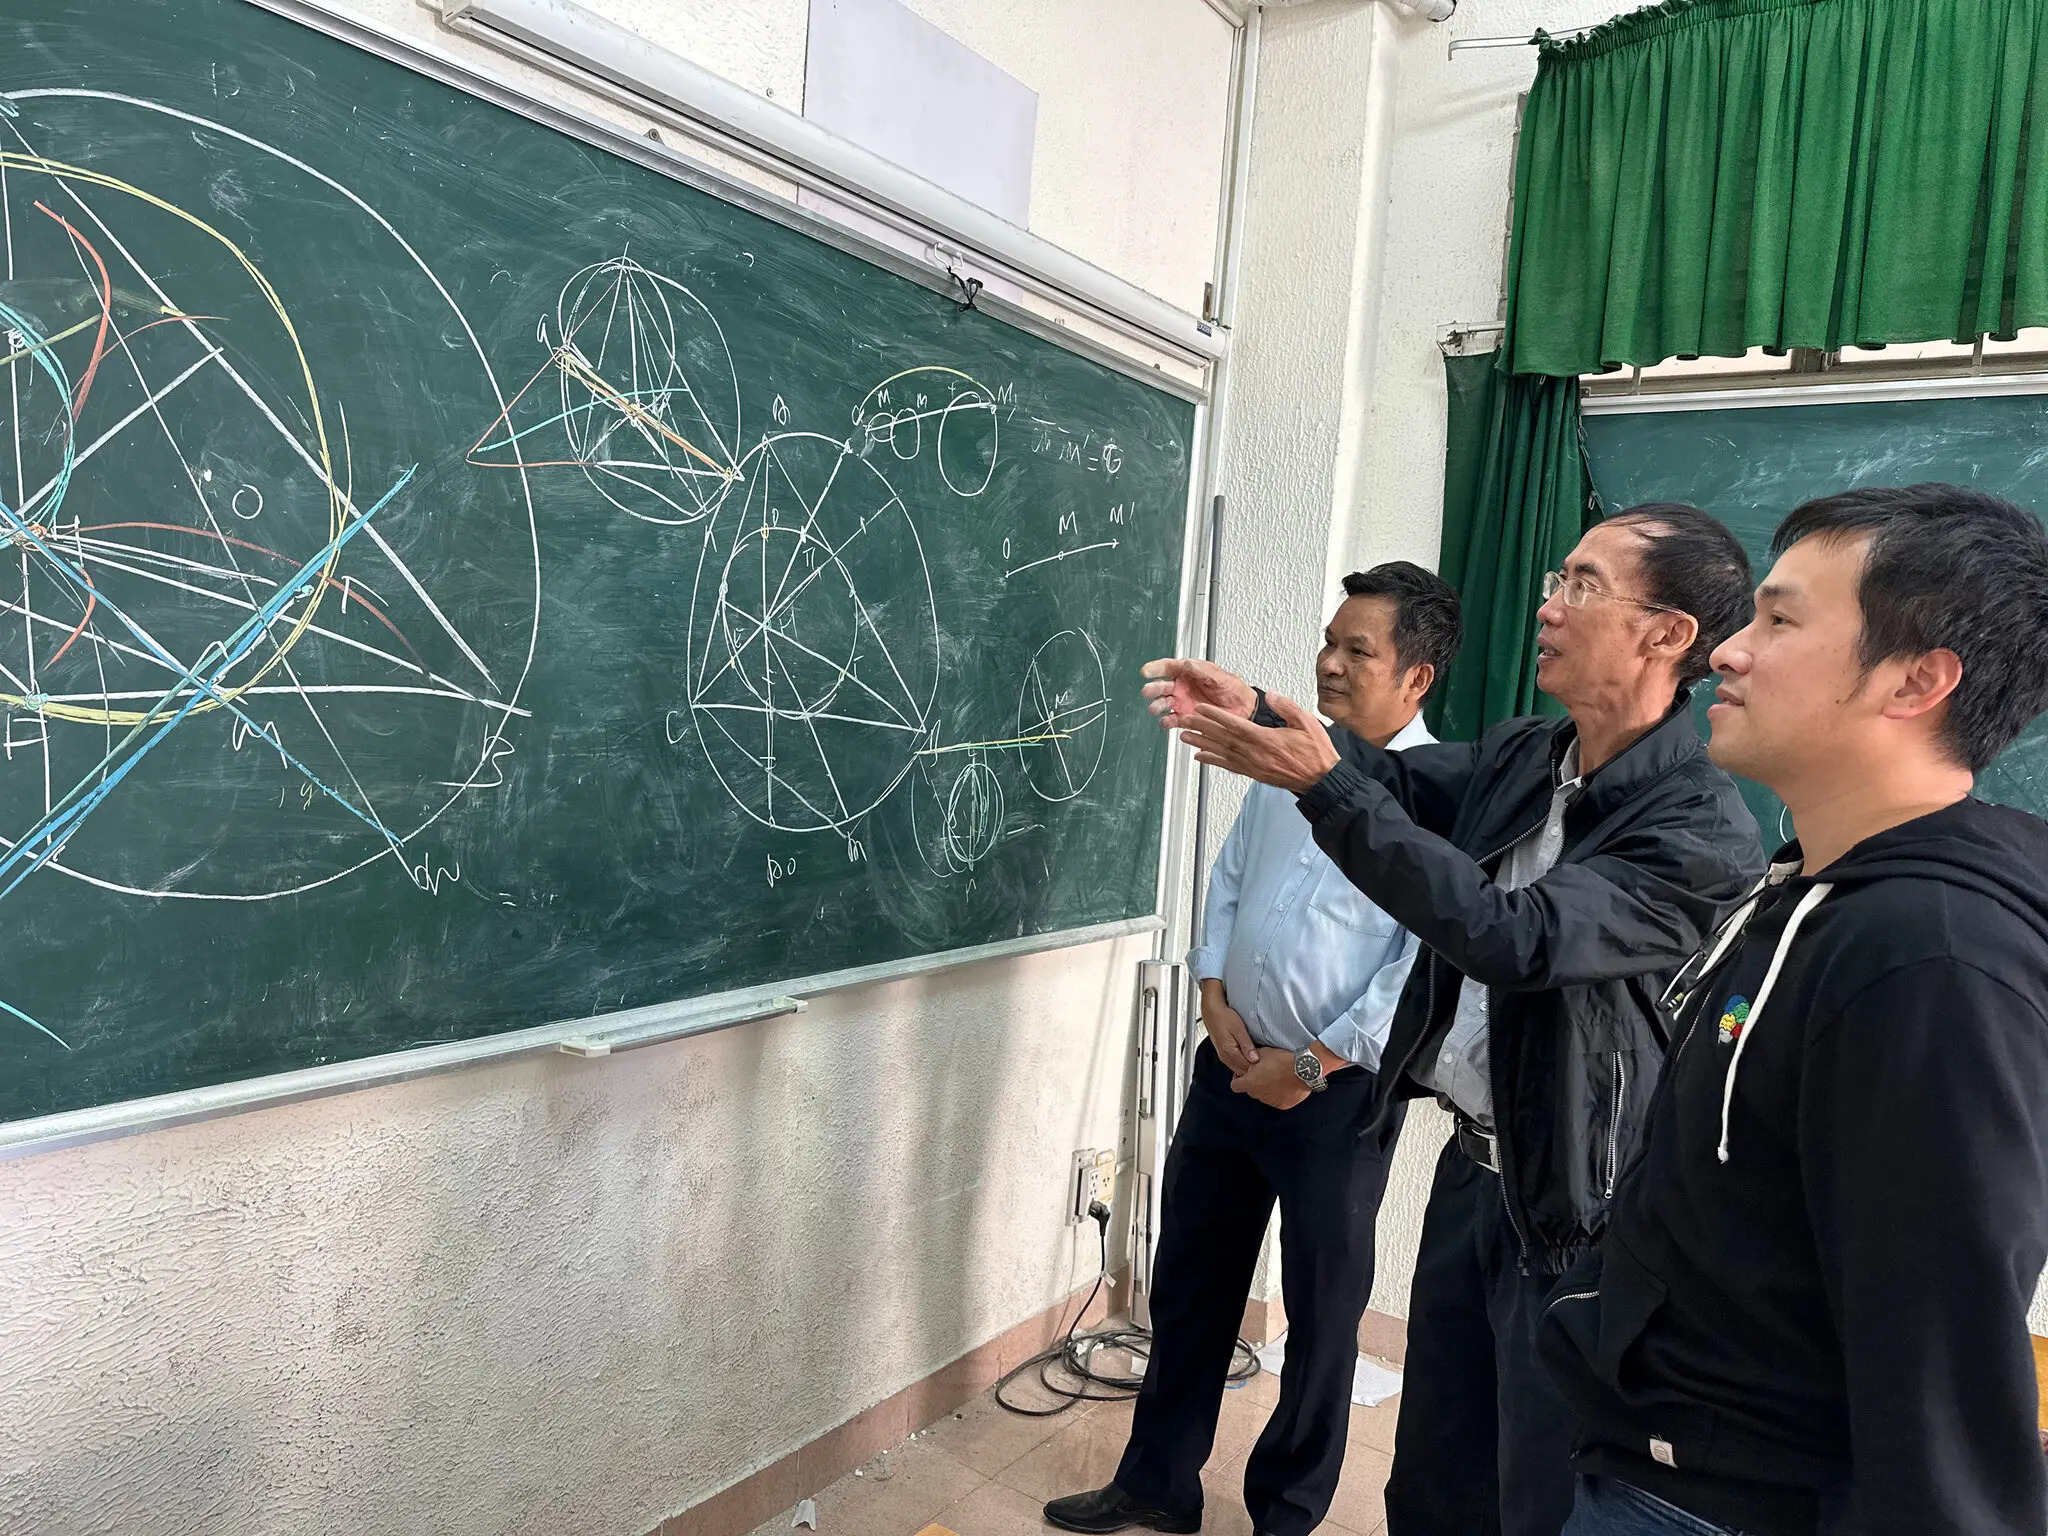
\includegraphics[width= 1\linewidth]{geometers.jpg}
		\caption{\small\textit{\color{timhieukhoahoc}Hình $7$: Trái qua phải: TS. Trần Nam Dũng, TS. Lê Bá Khánh Trình và TS. Lương Quốc Thắng. Nguồn: Wendy Nguyen.}}
		\vspace*{-10pt}
	\end{figure}
	\textbf{\color{timhieukhoahoc}Những mục tiêu tiếp theo}
	\vskip 0.1cm
	Từ lâu, lý luận toán học được xem là nền tảng của sự thông minh. Sau những thành công của các chương trình AI như AlphaGo của Google Deepmind trong cờ vây, mục tiêu tiếp theo của các nhà khoa học là xây dựng một hệ thống AI mạnh mẽ với khả năng lý luận nâng cao đủ khả năng giành huy chương vàng Olympiad. Về lâu dài, các nhà nghiên cứu hướng tới việc xây dựng các hệ thống AI có thể khái quát hóa trên các lĩnh vực toán học, phát triển khả năng giải quyết vấn đề và lý luận phức tạp mà các hệ thống AI nói chung sẽ phụ thuộc vào, đồng thời mở rộng biên giới kiến thức của con người.
	\vskip 0.1cm
	Nhằm thúc đẩy sự phát triển nghiên cứu theo hướng trên, tháng $11$ năm $2023$, XTX Markets, một công ty giao dịch thuật toán \footnote[4]{\color{timhieukhoahoc}Áp dụng các thuật toán học máy để thiết lập tự động hoặc đưa ra khuyến nghị cho các giao dịch.} đa quốc gia có trụ sở tại London, đã công bố giải thưởng AI Mathematical Olympiad Prize trị giá 5 triệu USD dành cho hệ thống AI nào giành được huy chương vàng tại IMO. Thành công của AlphaGeometry có thể được xem là một bước tiến quan trọng. Sự kết hợp sáng tạo giữa mô hình ngôn ngữ lớn hiện đại với công cụ suy luận biểu tượng truyền thống cùng với tiềm năng của việc đào tạo hệ thống AI từ đầu bằng dữ liệu tổng hợp quy mô lớn có thể mở ra cách tiếp cận mới cho các hệ thống AI trong tương lai. 
	\vskip 0.1cm
	Dù không thể phủ nhận những tiến bộ ấn tượng về khả năng đưa ra kết luận và giải quyết các vấn đề toán học của AI so với các cách tiếp cận truyền thống nhưng AlphaGeometry vẫn cho thấy những hạn chế nhất định. 
	\vskip 0.1cm
	Trước hết, AlphaGeometry chỉ tập trung vào các bài hình học phẳng Euclid và loại trừ các chủ đề như bất đẳng thức hình học và hình học tổ hợp. Từ lâu, hình học Euclid được biết đến như là một nền tảng thử nghiệm lý tưởng cho lý luận tự động vì nó tạo thành một miền khép kín với các quy tắc cố định. Điều này rất khác với các lĩnh vực khác như Đại số, Số học, Tổ hợp hay Giải tích. \footnote[5]{\color{timhieukhoahoc}Nhà toán học Alfred Tarski đã chứng mình rằng hình học phẳng Euclid cổ điển là nhất quán, đầy đủ và có thể quyết định được: mọi mệnh đề trong ngôn ngữ của nó đều có thể được chứng minh hoặc bác bỏ từ các tiên đề, và tồn tại có một thuật toán quyết định xem một khẳng định có thể được suy ra một cách cơ học từ các tiên đề hay không.}
	\vskip 0.1cm
	Bên cạnh đó, việc phụ thuộc vào các công cụ biểu tượng để tạo ra dữ liệu tổng hợp khiến cho việc áp dụng ý tưởng của AlphaGeometry cho các lĩnh vực khác cũng như các lĩnh vực khác trong toán học không dễ dàng. Việc thiếu dữ liệu huấn luyện hình học đa dạng đã hạn chế khả năng suy luận phức tạp cần thiết cho các bài toán nâng cao. Việc phụ thuộc vào một công cụ biểu tượng được đặc trưng bởi các quy tắc nghiêm ngặt có thể hạn chế tính linh hoạt, đặc biệt là trong các tình huống giải quyết vấn đề trừu tượng hoặc độc đáo. Việc giải quyết những hạn chế này sẽ rất quan trọng để cải thiện khả năng ứng dụng của AlphaGeometry trong các lĩnh vực toán học khác nhau.
	\vskip 0.1cm
	Tác động của AlphaGeometry đối với nghiên cứu AI và toán học vẫn chưa được nhìn thấy, nhưng công trình này chắc chắn mang lại một số ý tưởng và nguồn cảm hứng mới cho các lĩnh vực này. 
	\vskip 0.1cm
	Nhìn về phía trước, TS. Trịnh Hoàng Triều và các đồng nghiệp cam kết nghiên cứu những thách thức còn lại và xác định các cơ hội để tiến bộ, với mục đích cuối cùng là nâng cao năng lực giải quyết vấn đề của AI. Công việc của họ là minh chứng cho hành trình khám phá và đổi mới đang diễn ra trong sự giao thoa giữa trí tuệ nhân tạo và toán học.
	\vskip 0.1cm
	\textbf{\color{timhieukhoahoc}Tài liệu}
	\vskip 0.1cm
	[$1$] Trinh, T.H., Wu, Y., Le, Q.V. et al. \textit{Solving olympiad geometry without human demonstrations}. Nature $625$, $476-482$ ($2024$).
	\vskip 0.1cm
	[$2$] \textit{AlphaGeometry: An Olympiad--level AI system for geometry}, Google DeepMind's blog, $17.01.2024$.
	\vskip 0.1cm
	[$3$] \textit{A.I.’s Latest Challenge: the Math Olympics}, The New York Times, $17.01.2024$.
	\vskip 0.1cm
	[$4$] Greenberg, Marvin Jay. \textit{Old and New Results in the Foundations of Elementary Plane Euclidean and Non--Euclidean Geometries}, The American Mathematical Monthly. $117$ $(3):$ $198$ ($2010$).
\end{multicols}


